\documentclass[12pt]{extarticle}
\usepackage[utf8]{inputenc}
\usepackage{cite}
\usepackage{indentfirst}
\usepackage{graphicx}

\title{Answering Invalid TLD Requests at Line Rate with DPDK}
\author{Haoda Wang}
\date{May 2020}

\begin{document}

\maketitle

\section{Program Design}
The program was based on DPDK's KNI example application, which mirrors traffic between a virtual KNI interface and a physical one assigned to DPDK. This also provides a modest increase in performance under normal usage by eliminating some expensive system calls. This comes at the cost of dedicating some cores purely to DPDK. \\

As the KNI interface exists as a standard Ethernet device, the application can be transparent to both the client and the server. Any operations on the interface will have the same result as if it was done to the physical interface. This is useful as all queries containing valid top-level domains can be processed normally. \\

Unlike DPDK's KNI example, this application requires four threads per interface to run at maximum efficiency. In addition, it uses two additional ring buffers to minimize packet loss. One of the threads moves all incoming packets into the \texttt{ETH\_RX\_RING} buffer. \\

Another thread then reads the packets in the \texttt{WORKER\_RX\_RING} buffer, where the following properties of the packet is determined:

\begin{enumerate}
  \item Is this host the destination for the packet?
  \item Is this packet a UDP packet going to port 53?
  \item Is this packet a standard DNS query?
  \item Does this packet contain an invalid TLD?
\end{enumerate}

If the answer to one of the above questions is "no", the packet is immediately moved into the \texttt{KNI\_RX\_RING}, at which point it is processed by the host. However, if the answers to all the questions is "yes", then the packet may be part of an invalid TLD attack, and is moved to the \texttt{WORKER\_TX\_RING}. \\

The third thread takes the packets in \texttt{WORKER\_TX\_RING} and modifies them into NXDOMAIN replies. This is done by swapping the destination and source addresses and ports in the Ethernet, IPv4, and UDP headers. Then, the DNS headers are changed so that the request becomes an authoritative answer. Then the IP checksum is calculated and set, and the packet is put into the \texttt{ETH\_TX\_RING}, where the NIC will send it out. \\

The final thread takes all outgoing traffic from the \texttt{KNI\_TX\_RING} buffer and moves them to the \texttt{ETH\_TX\_RING}. A visualization of the program's architecture can be shown below: \\

\noindent
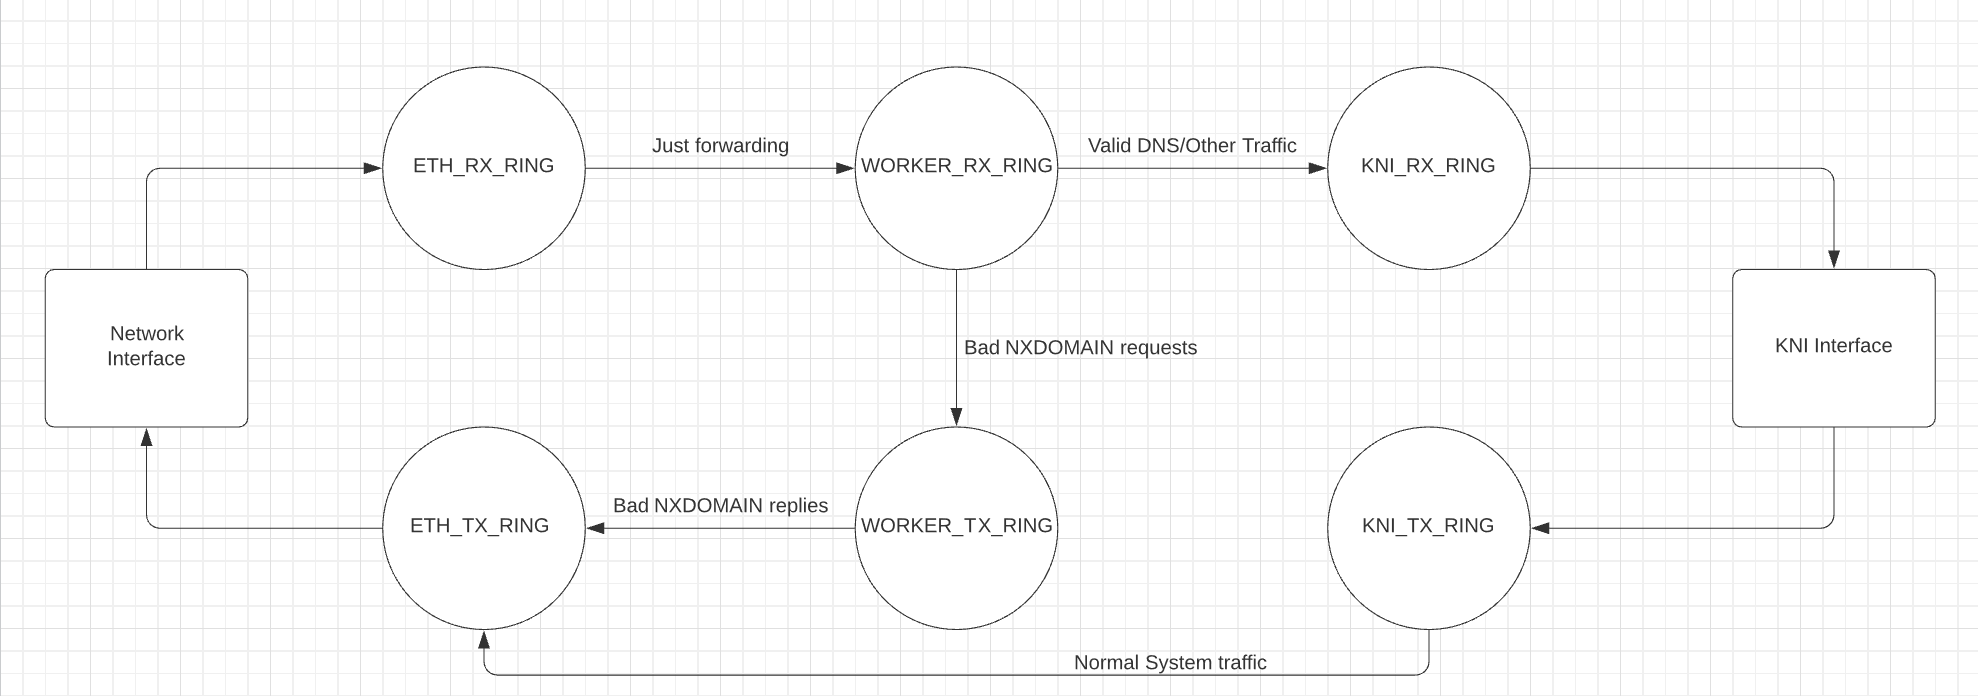
\includegraphics[width=\textwidth]{buf_layout.png}

\section{Test Setup}
The application was tested using a pair of d430 nodes on Emulab, which contains an Intel X710 10GbE network card. All nodes ran Ubuntu 18.04. Each node had tuned-adm running with the network-throughput profile loaded. \\

One of the nodes was designated as a root node, and had the Bind9 DNS server installed and configured according to the configuration generator at \texttt{localroot.isi.edu}. However, to avoid interfering with legitimate DNS servers, all external master nodes were removed. \\

The \texttt{testing/generate\_bind\_config.py} script in the Git repository was used to generate 200,000 random DNS entries with a randomly selected TLD from ICANN's list of valid TLDs, and a randomly generated UUID as a domain name. The generation script also creates an input file for dnsperf with every valid TLD generated by the script. \\

Tests were done using both dnsperf and DPDK-pktgen. In both cases, 600,000 requests were sent, either using the valid TLDs generated from the bind9 config or invalid, randomly generated UUIDs. As each request is a single packet, the DPDK-pktgen tests assumed that each packet was a request. \\

\section{Results}

The following results are from a dnsperf run using invalid TLDs. The run simulated 1000 DNS clients and ran on 12 threads, with a timeout of 5 seconds. Each client sends requests and waits for a reply before sending the next one. The timeout applies to dropped packets as well, so each dropped packet incurs a penalty of 5 seconds on the DNS client that requested it. \\

\begin{center}
\begin{tabular}{ ||c|c|c|| }
\hline
Attack Traffic & With dns-proxy & Without dns-proxy \\
\hline
Queries sent & 600,000 & 600,000 \\
Queries completed & 59,7829 & 600,000 \\
Queries lost & 2,171 & 0 \\
Run time (s) & 107.773797 & 182.762914 \\
Queries per second & 5,547.071892 & 3,282.941746 \\
Average Latency (s) & 0.000097 & 0.030340 \\
Minimum Latency (s) & 0.000017 & 0.002217 \\
Maximum Latency (s) & 0.000657 & 1.122642 \\
Latency StdDev (s) & 0.000031 & 0.030501 \\
\hline
\end{tabular}
\end{center}

The results below show the performance against dnsperf using legitimate traffic. The configuration is identical to the one above, with only the input file changed. \\

\begin{center}
\begin{tabular}{ ||c|c|c|| }
\hline
Legitimate Traffic & With dns-proxy & Without dns-proxy \\
\hline
Queries sent & 600,000 & 600,000 \\
Queries completed & 599,750 & 599,850 \\
Queries lost & 250 & 150 \\
Run time (s) & 35.888684 & 23.945254 \\
Queries per second & 16,711.39572 & 25,050.893175 \\
Average Latency (s) & 0.00373 & 0.00254 \\
Minimum Latency (s) & 0.000117 & 0.000112 \\
Maximum Latency (s) & 0.039361 & 0.334216 \\
Latency StdDev (s) & 0.003353 & 0.010643 \\
\hline
\end{tabular}
\end{center}

To ensure that packets can be replied to at line rate, DPDK-pktgen was able to send all 600,000 packets at 1.3Mpps and record all 600,000 packets returned. \\

\end{document}
